\documentclass[10pt]{article}
%%%packages%%%
%\usepackage[latin1]{inputenc}
%\usepackage{newcent}
\usepackage{graphicx}
\usepackage{amsmath}
\usepackage{amsfonts}
\usepackage{amssymb}
\usepackage{amsthm}
\usepackage{listings}%R Code
\usepackage{color}%R code
% \usepackage{tkz-graph}
% \usepackage{tkz-berge}
% \usepackage{tkz-euclide}
\usepackage{hyperref}
%\usepackage[left=1in, right=1in, top=.9in, bottom=.9in]{geometry}
\usepackage{setspace}
%\usepackage{hyperref}
\usepackage{pdflscape}
%%%theoerms, etc%%%%
\theoremstyle{plain}% default
\newtheorem{thm}{Theorem}[section]
\newtheorem{prop}{Proposition}[section]
\newtheorem{lem}{Lemma}[section]
\newtheorem{pf}{Proof}[section]
\theoremstyle{definition}
\newtheorem{definition}{Definition}[section]
\newtheorem{example}{Example}[section]
\theoremstyle{remark}
\newtheorem{rmk}{Remark}[section]
\newtheorem{case}{Case}
\newtheorem{prob}{Problem}[section]
%%%% R Code%%%%
\definecolor{dkgreen}{rgb}{0,0.6,0}
\definecolor{gray}{rgb}{0.5,0.5,0.5}
\definecolor{mauve}{rgb}{0.58,0,0.82}
\lstset{frame=tb,
  language=R,
  aboveskip=3mm,
  belowskip=3mm,
  showstringspaces=false,
  columns=flexible,
  basicstyle={\small\ttfamily},
  numbers=none,
  numberstyle=\tiny\color{gray},
  keywordstyle=\color{blue},
  commentstyle=\color{dkgreen},
  stringstyle=\color{mauve},
  breaklines=true,
  breakatwhitespace=true
  tabsize=3
}
%%%%%%%%custom commands
\newcommand{\bbH}{{\mathbb{H}}}
\newcommand{\bbR}{{\mathbb{R}}}
\newcommand{\bbP}{{\mathbb{P}}}
\newcommand{\bbZ}{{\mathbb{Z}}}
\newcommand{\bbC}{{\mathbb{C}}}
\newcommand{\bbQ}{{\mathbb{Q}}}
\newcommand{\bbA}{{\mathbb{A}}}
\newcommand{\bbF}{{\mathbb{F}}}
\newcommand{\bbh}{{\mathbb{H}}}
\newcommand{\bbr}{{\mathbb{R}}}
\newcommand{\bbp}{{\mathbb{P}}}
\newcommand{\bbz}{{\mathbb{Z}}}
\newcommand{\bbc}{{\mathbb{C}}}
\newcommand{\bbq}{{\mathbb{Q}}}
\newcommand{\bba}{{\mathbb{A}}}
\newcommand{\bbf}{{\mathbb{F}}}
\newcommand{\bbn}{{\mathbb{N}}}
\newcommand{\bbN}{{\mathbb{N}}}
\newcommand{\disteq}{{\overset{D}{=}}}
\newcommand{\cross}{{\times}}
\newcommand{\CBeta}{{  \left( \begin{array}{c}\hat{\beta}_{1,1} - \hat{\beta}_{2,1} \\ \hat{\beta}_{1,2} -
\hat{\beta}_{2,2} \\ \vdots \\ \hat{\beta}_{1,p} - \hat{\beta}_{2,p}    \end{array} \right) }}
\newcommand{\COVW}{{\left[ \begin{array}{cc}\sigma_1^2 \left( X_1 ' X_1\right)^{-1}\\ \sigma_2^2 \left( X_2 '
X_2\right)^{-1} 
\end{array} \right]}}
\newcommand{\MSRES}{{\sigma_1^2 n_1 + \sigma_2^2 n_2 - p \left( \sigma_1^2 + \sigma_2^2 \right) }}
\newcommand{\XX}{{\left(X ' X\right)^{-1} }} 
\newcommand{\xx}{{\left(X ' X\right)^{-1} }} 
\newcommand{\ssres}{{\text{SS}_\text{RES}}}
\newcommand{\inv}[1]{{#1^{-1}}}
% \newcommand{\iff}{{\Leftrightarrow}}
\newcommand{\comp}[2]{{\left( #1 \circ #2\right) }}
\newcommand{\set}[2]{{\left\lbrace \left.  #1 \left\vert #2  \right.\right.\right\rbrace  }}
\newcommand{\topo}{{\mathcal{T}}}
\newcommand{\powset}[1]{{\mathcal{P}\left( #1 \right) }}
%\newcommand{\vec}[1]{{\overrightarrow{#1} }}
%%%%Spacing commands %%%%%
\newcommand{\tab}{\hspace{.4cm}}
\newcommand{\quadtab}{\hspace{.4cm}}
\newcommand{\matab}{\hspace{1.01600mm}}
\renewcommand{\arraystretch}{1.5}
\newcommand{\RNum}[1]{\lowercase\expandafter{\romannumeral #1\relax}}
\newcommand{\rn}[1]{\lowercase\expandafter{(\romannumeral #1\relax)}}
\newcommand{\floor}[1]{\left\lfloor #1 \right\rfloor}
\newcommand{\ceil}[1]{\left\lceil #1 \right\rceil}
\newcommand{\combo}[2]{\left(\begin{array}{c}#1\\#2\end{array}\right)}
%\renewcommand{\baselinestretch}{1.0}
% 1.0 is for one line space, 2.0 is for double-line space, etc
%%%%Spacing commands %%%%%

%%%%Margins%%%%%% - Clinton Bowen
%%Please refer to http://en.wikibooks.org/wiki/LaTeX/Page_Layout
%%The parameters below are described pictorally on this webpage.  Tinker with the settins as needed.
\setlength{\evensidemargin}{0cm}
\setlength{\oddsidemargin}{0pt}
\setlength{\topmargin}{.5in}
\setlength{\hoffset}{0in}
\setlength{\voffset}{0in}
\setlength{\headheight}{0pt}
\setlength{\headsep}{0in}%should be 1 inch from header titles
\setlength{\textheight}{21cm}
\setlength{\textwidth}{15.5cm}
\setlength{\marginparsep}{0pt}
\setlength{\marginparwidth}{0pt}
\setlength{\footskip}{0pt}
%%%%Margins%%%%%% - Clinton Bowen
\author{Clinton Bowen}
\title{Thesis Draft}
\date{November 30, 2013}
\makeindex
\begin{document}
\maketitle
\begin{abstract}
We look into the decidability of whether a hinged configuration locks.
\end{abstract}
\section{Introduction}
We look into the decidability of continuity on planar configuration space using regular, unitary hexagonal polygons.  These polygons can also represent unit disk configurations \cite{Breu19983} 
\begin{figure}[ht]
\begin{center}
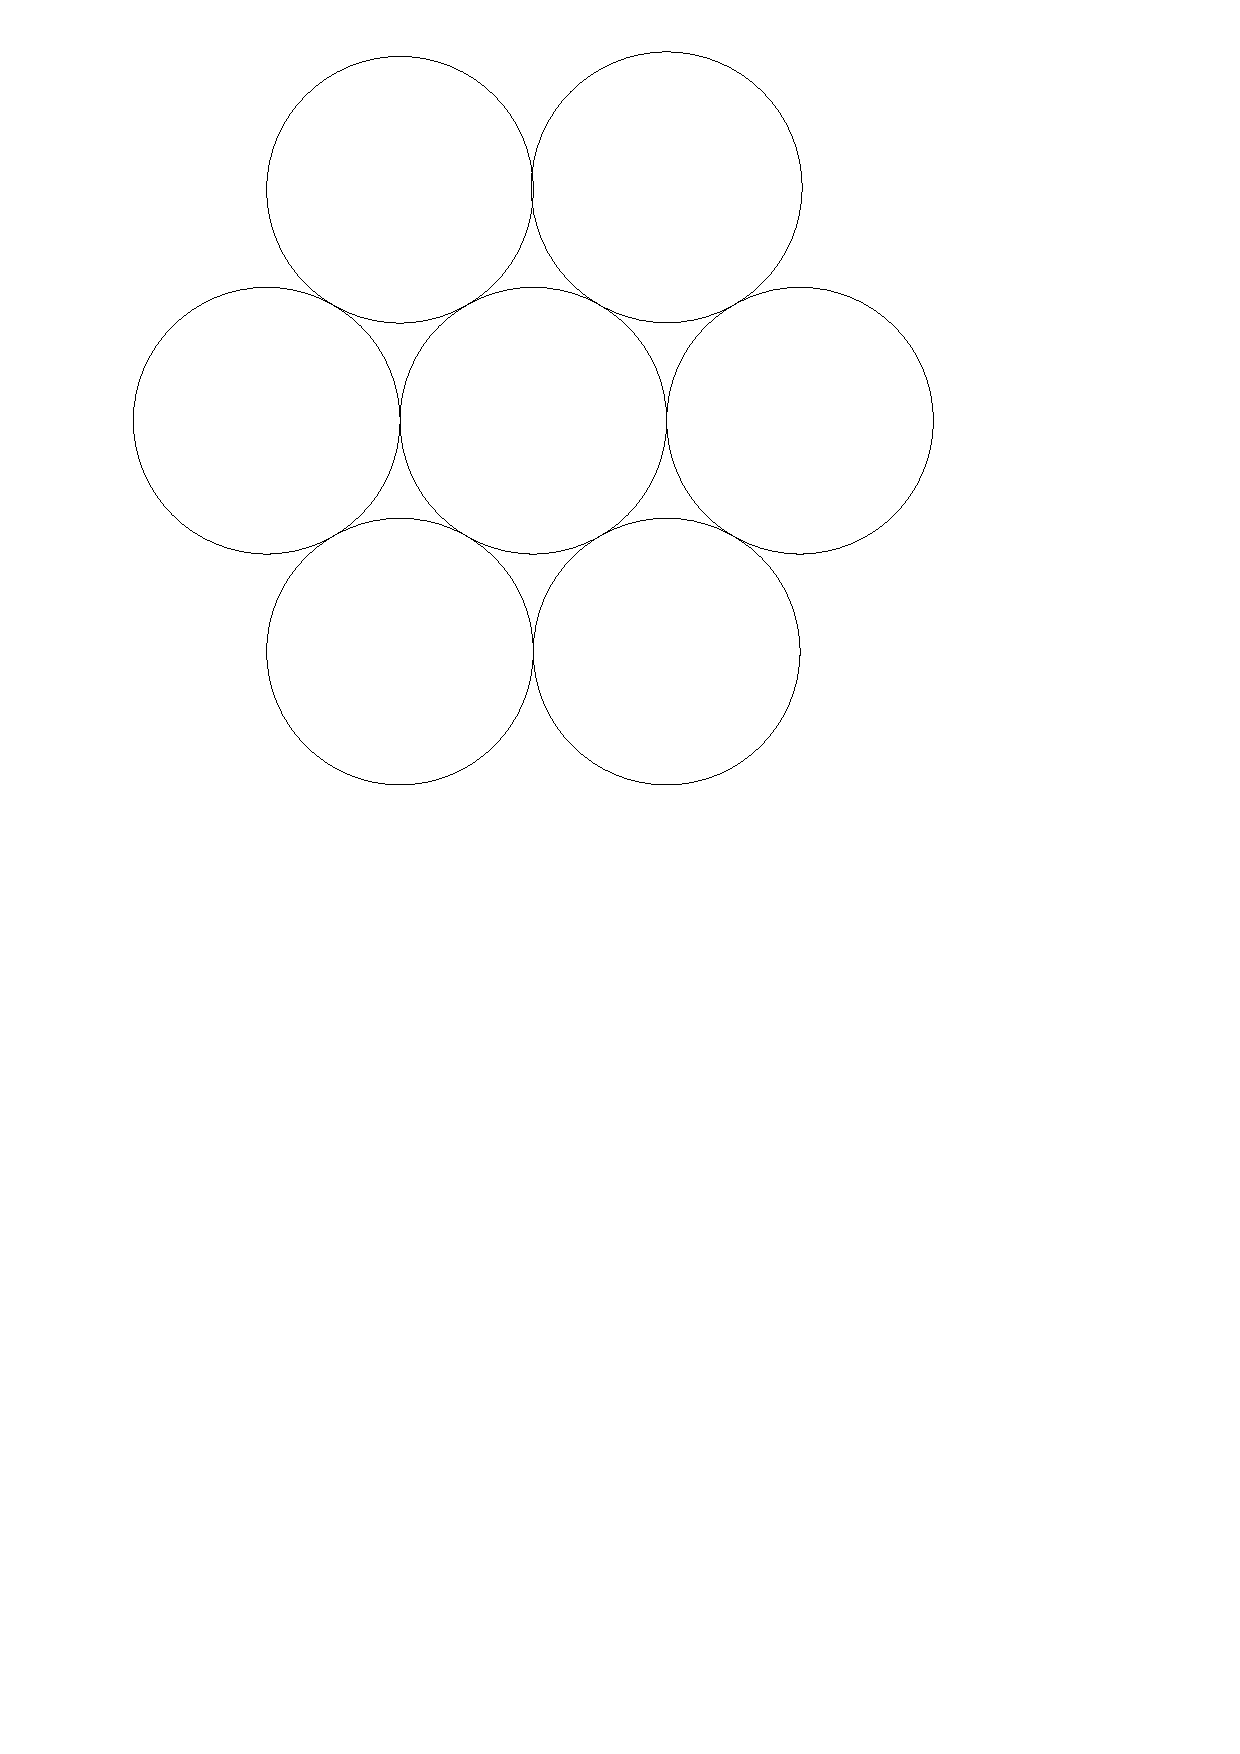
\includegraphics{graphics/7ballLocked.pdf}
\caption{A locked 7 ball configuration}
\label{figure:7ballLocked}
\end{center} 
\end{figure}
% We need the following:
% \begin{itemize}
% \item[\rn{1}] discussion on the outer configuration of hexagons
% \item[\rn{2}] discussion on the inner configuration (lattice tesselation) of hexagons the convex hull of \rn{1}
% \item[\rn{3}] discussion on the hinged cells that reside in the boundary of \rn{2}
% \item[\rn{4}] discussion on the lockedness of \rn{3} where it has two modes (boolean variable)
% \item[\rn{5}] the area of interests:
% \begin{itemize}
% \item how big are the cells of \rn{3}?
% \item does cell size matter in \rn{3}?
% \item How to form a 3-sat conjunction from a set of cells at corners of the individual hexagons within the tesselation
% \item how to form a conjunction from a set of cells on the edges of the of the hexagons.
% \end{itemize} 
% \end{itemize}  
\paragraph{Motivation}
Protein folding, graphite, crystalline structures in metallurgy.
\paragraph{Outline}
Section 2 covers the necessary mathematical concepts to understanding the
problem.  Section 3 explains the problem, Section 4 covers the results and
findings about the problem.  Section 5, the conclusion, offers final remarks on
the problem.

\chapter{Background}

We consider four decision problems surrounding graph theory and geometry. 
The graph theory based problems involve polygonal linkages and the geometry based problems involve something called a contact graph of disks.  
In each problem, we decide whether a polygonal linkage or contact graph has a certain realization in the plane.

This thesis first presents preliminary information needed to pose our four problems, then we formally pose each problem and then provide the hardness results in all four cases.
We show that all four problems are intractable, or $\NP$ hard (see definition below). 

\section{Problem}
\subsection{Problem Statement} text
\subsection{Decidability of Problem} test
\subsection{Locked Configuration}
Test
\begin{figure}[ht]
\begin{center}
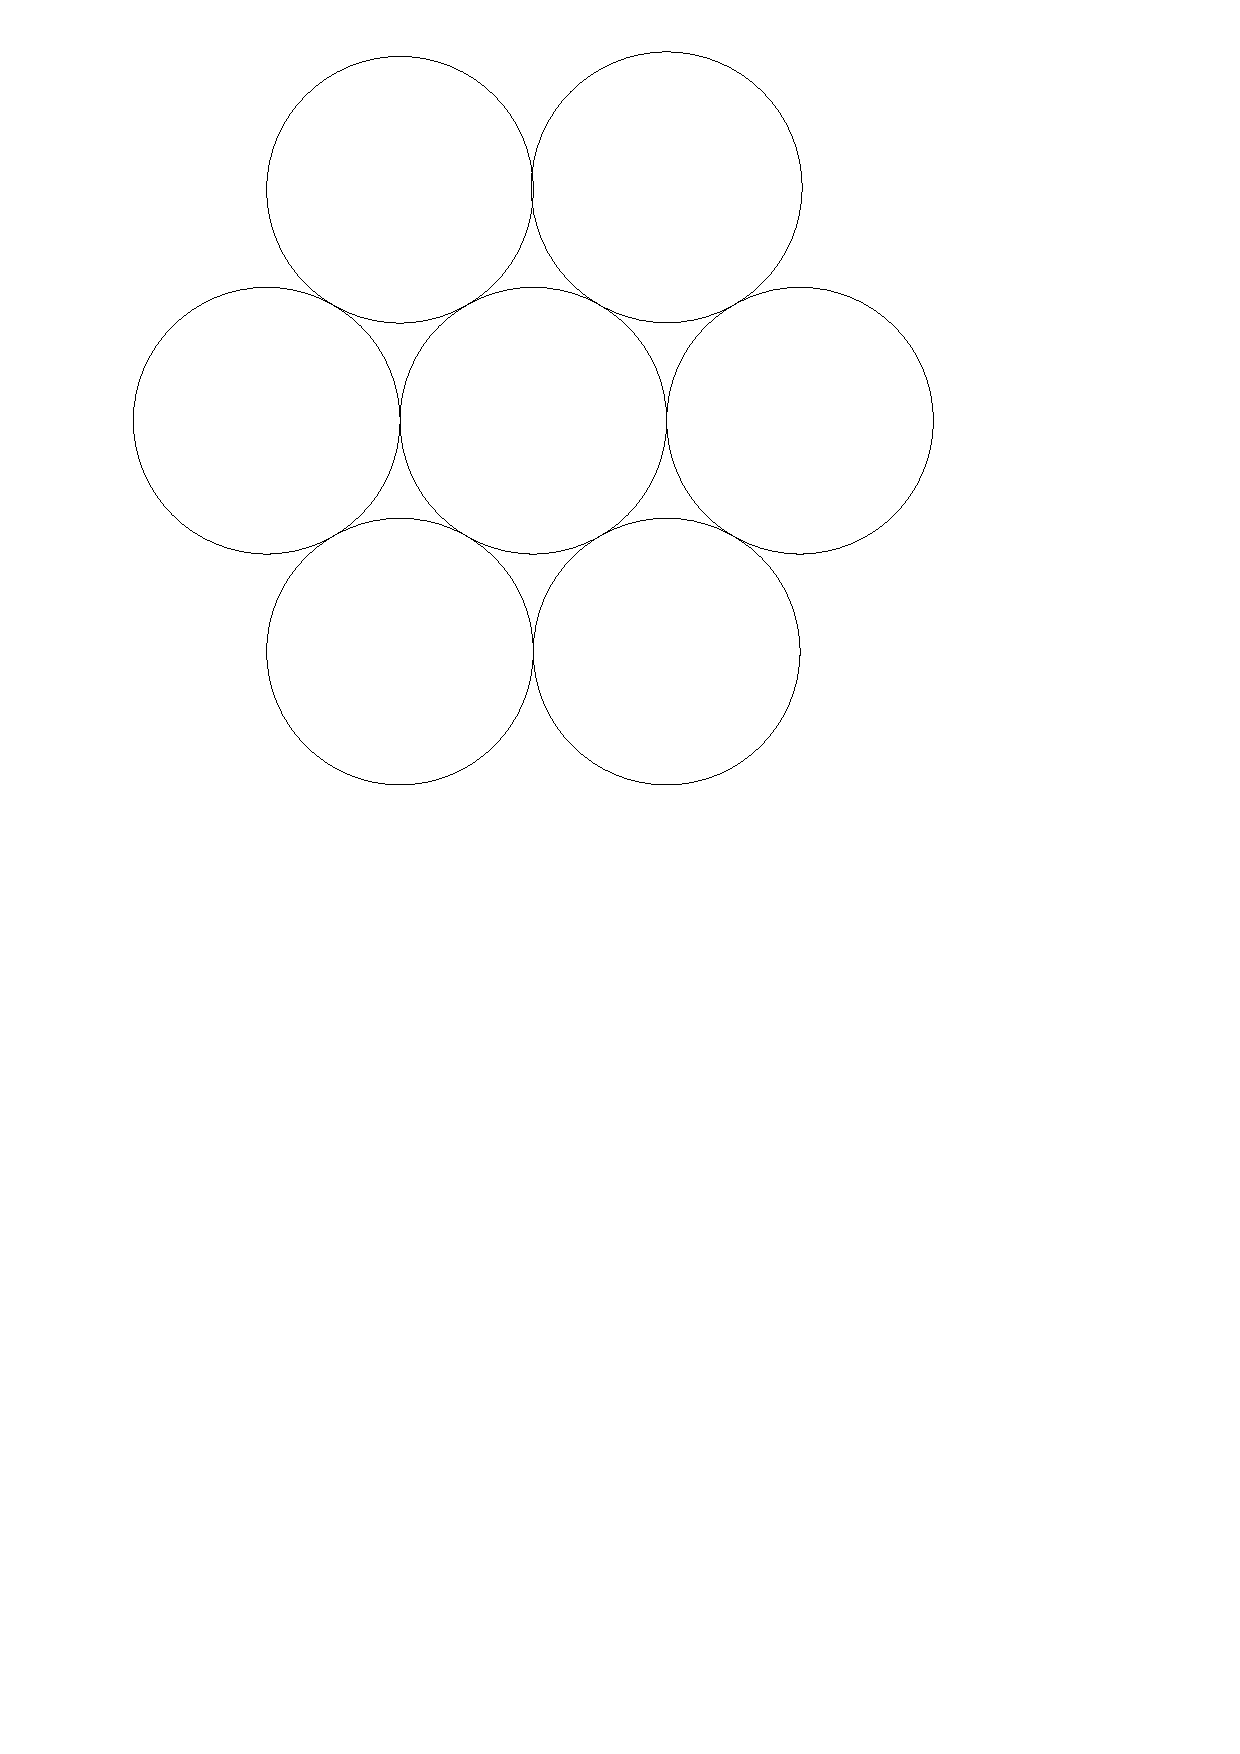
\includegraphics{graphics/7ballLocked.pdf}
\caption{A locked 7 ball configuration}
\label{figure:7ballLocked}
\end{center} 
\end{figure}
\begin{figure}[ht]
\begin{center}
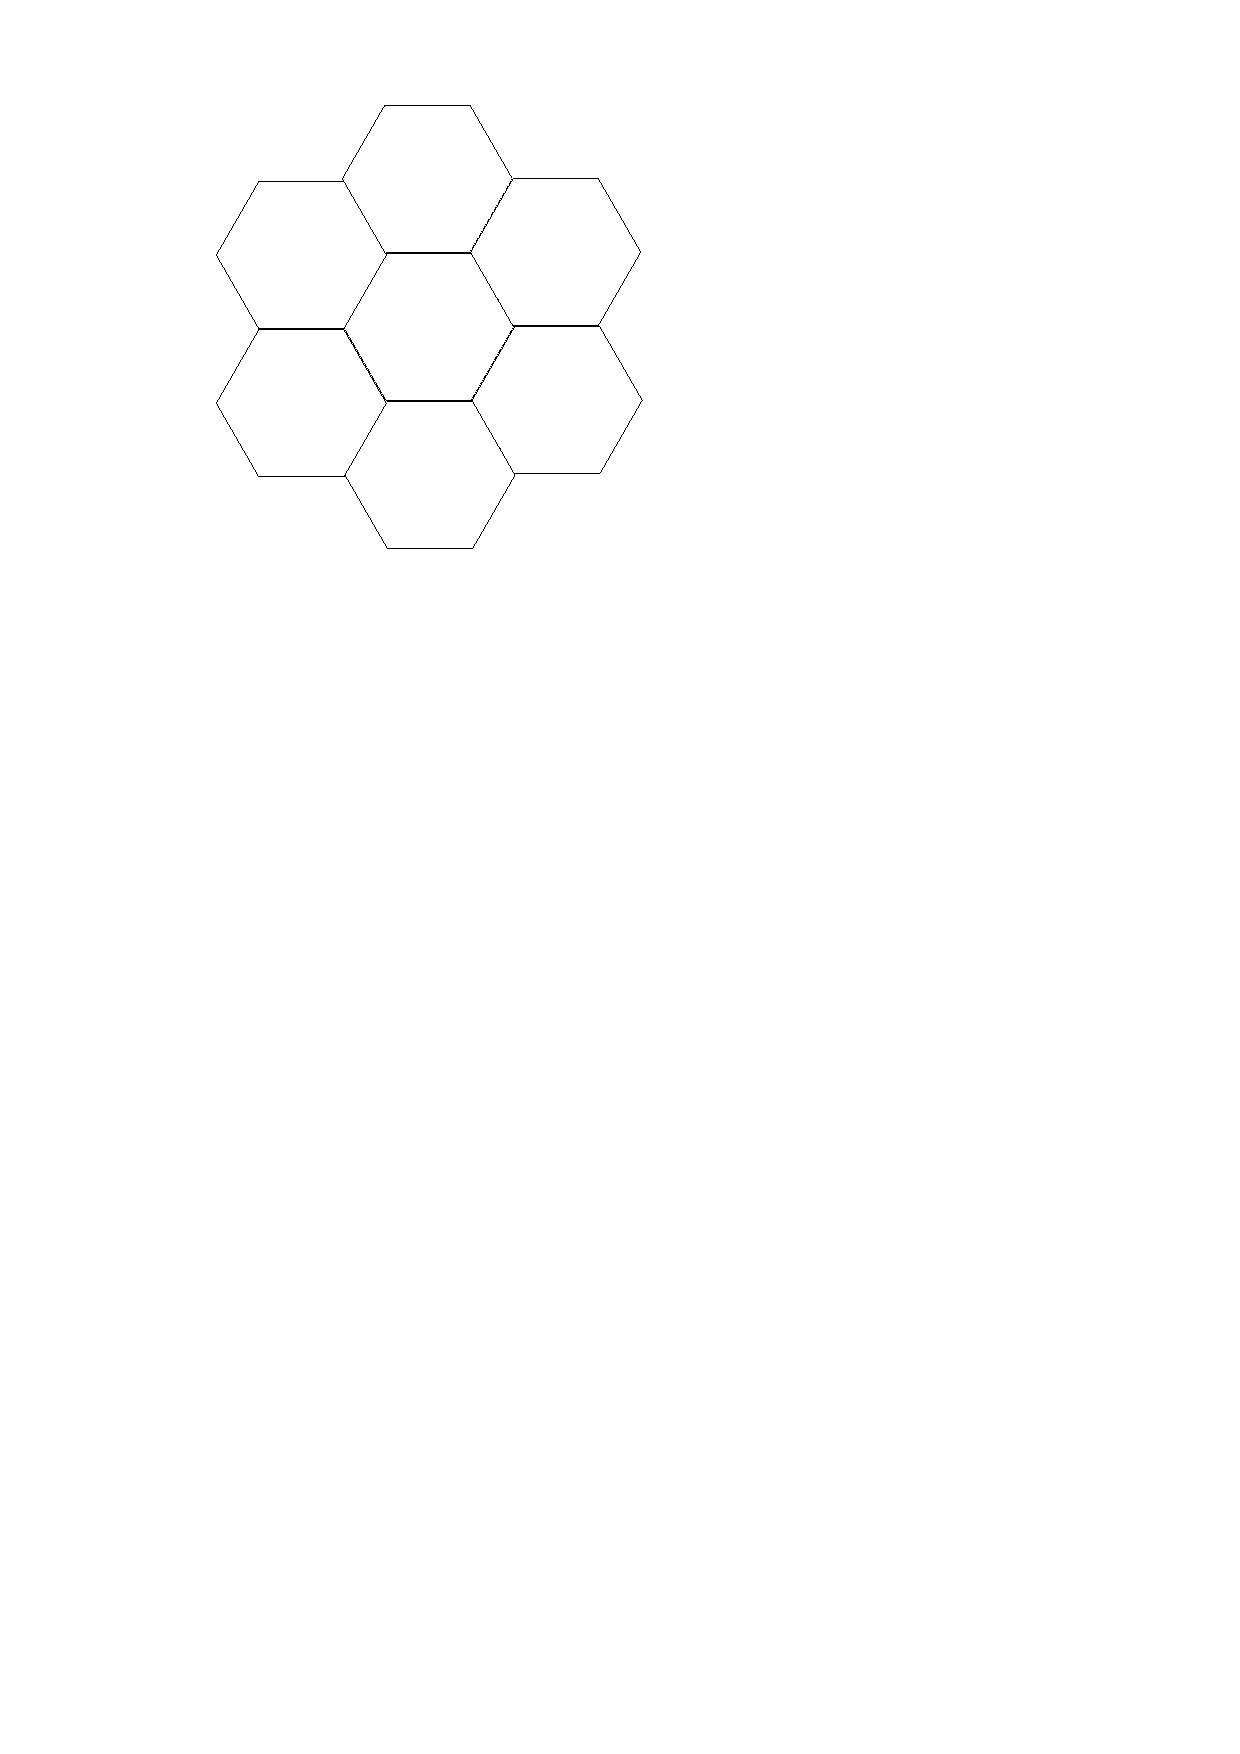
\includegraphics{graphics/7hexLocked.pdf}
\caption{A locked 7 ball configuration}
\label{figure:7hexLocked}
\end{center} 
\end{figure}
\newpage
\input{solution}
\section{Conclusion}
\nocite{demaine2008geometric,frederickson1997dissections,stephenson2005introduction}
\bibliographystyle{plain}
\bibliography{bibliography}
\end{document}